\section{Node Operations} \label{sec:node-operations}

Aside from handling incoming data operations, a Hydra node has other responsibilities partly due to being in a distributed, federated system and partly due to managing its own resources.

\subsection{Node Security Bootstrapping - AlexA/Proyash/Tianyuan}
\label{sec:nodeop-boostrap}
Similar to the user bootstrapping (Section~\ref{sec:dataop-bootstrap}), each Hydra node need to obtain its trust anchor, trust policies and certificate.

% The Hydra NOC performs multiple functions such as~(i) add/authorize a new hydra node~(ii) manage trust policies for the Hydra system etc.
In Hydra, each node obtains the trust anchor and initial trust policies out-of-band.
After that, Hydra NOC authenticates and authorizes each node on their node names and public keys.
This requires Hydra NOC knowing trustworthy <node name, public keys> bindings via initial out-of-band trust relations (e.g., ssh, email).%\ty{I worried HTTPS would complicates the picture (need to have the CAs engaged) so I removed it}
% A node needs to be authorized first before it joins the system.
% In Hydra, a Network Operator Center (NOC) serves as the system trust anchor.
% To bootstrap a Hydra node, out-of-band verification is needed to authenticate the initial communication between the node and NOC.
% A node wishes to join the system, generates a key pair, and delivers the pair <node name, public key> to NOC to authorize this instance to operate.
% This transfer can happen in various ways (i.e., auth HTTPS, ssh, email, etc.)

For simplicity, Hydra uses email to establish the initial trust relations.
Before establishing a new node, the node operator emails the <node name, public key> binding to the NOC operator who configures the NOC application to authenticate the received binding.
% However, we are considering the email option right now for Hydra for simplicity purposes.
% Before establishing a new node, a node operator would send the <node name, public key> pair to the NOC operator via email and the NOC operator will keep this record locally. 

Hydra node utilizes NDNCERT~\cite{} to perform the public key authentication and obtains certificate from NOC.
The Hydra NOC first verifies if the hydra node has the membership in the system by checking its public key in the pre-configured trusted bindings, and it asks the node to perform the Proof-of-Possession Challenge where the node uses private key to sign a nonce to prove its public key possession.
Upon successful signature verification, Hydra NOC issues the new node with a certificate with the node name and public key obtained from trusted name-key bindings.
%\ty{I'm not sure people are referring to the NDNCERT PoP challenge here, pls reverse the revision if I'm wrong}
% However, a node still needs an NDN certificate to operate as an authorized Hydra node.
% A node uses/runs NDNCERT~\cite{} to get the actual certificate from NOC.
% When NOC receives a certificate request, t first checks whether this node is authorized to join or not by checking its locally kept record of trusted nodes to join.
% If yes, it uses the public key to encrypt a nonce (in the "challenge" part of NDNCERT) to determine the nodes' legitimacy. 

A Hydra node completes its security bootstrapping by obtaining and installing the issued certificate.
In Hydra, we assume that the NOC is trusted, and each Hydra node is also trusted after it completes the bootstrapping process. \ty{this should go into the threat model or security assumption}
\subsection{Federated Node Responsibilities}

\begin{figure}[!ht]
    \centering
    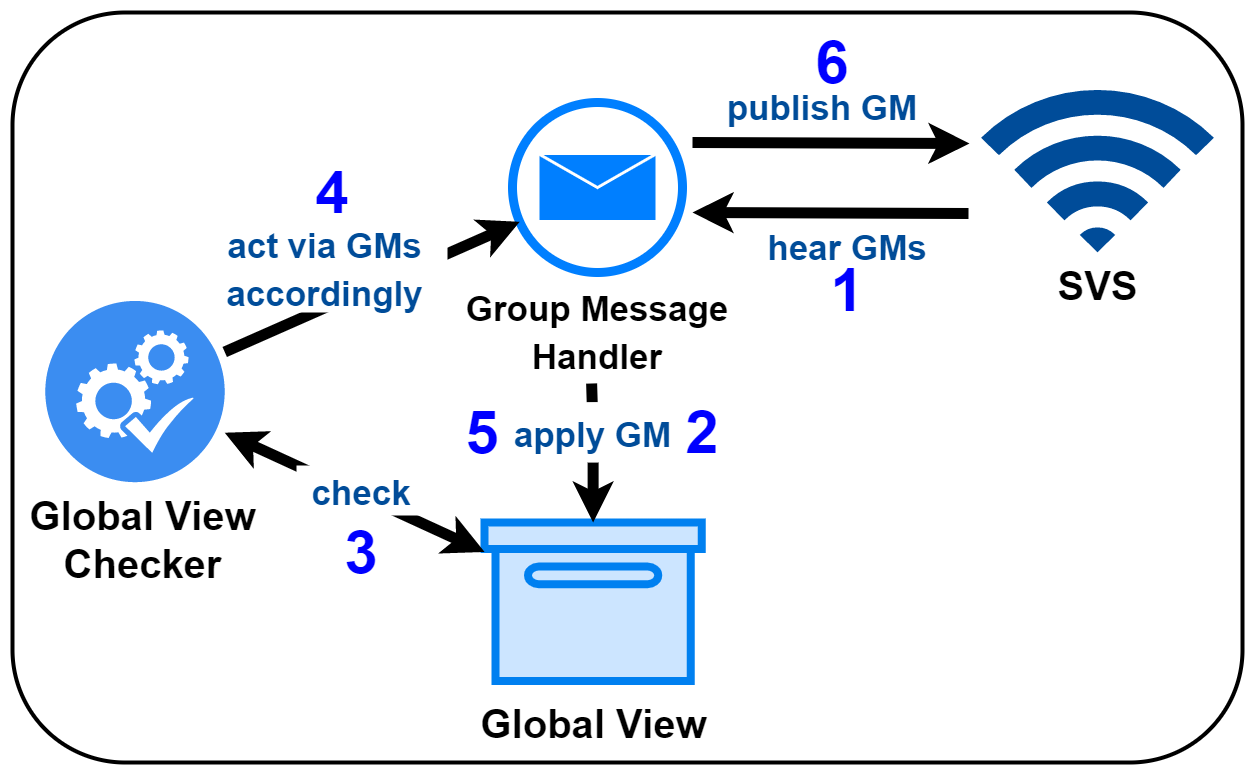
\includegraphics[width=\columnwidth]{visuals/checker-sys.png}
    \caption{Modules Involved with Checking the Global View}
    \label{fig:checker-sys}
\end{figure}

One of the major responsibilities that a node actively fulfills is checking if any federated actions are required to be taken. This is done by the Global View Checker. The Global View Checker consistently checks the Global View as seen in figure \ref{fig:checker-sys}.

\subsection{Storage Management}
Each node storage space contains two components: Local File Storage and Local Reserved Storage. Local File Storage provides sufficient space to support valid replication requests. The function of Local Reserved Storage is to reserve computational resources for system processes, this space is not used to store replication files or metadata for Hydra.

\subsection{Joining the federation and membership management}

%\todo[inline]{Need to expand. This is too brief.}
To join the federation a node must install hydra and begin broadcasting a heartbeat. Once the broadcasted heartbeat has been detected between the new node and one of the pre-existing nodes within the federation. The pre-existing node will update the global view for the federation to acknowledge the new node. At the same time, the new node is still broadcasting its heartbeat to other pre-existing nodes within the federation, and they are following suit with the previously discussed pre-existing node's actions. This will increase the propagation of the new node's acknowledgment within the global view. Once this is complete it will be listed as a node within the network or federation, and the others can begin to interact with the new node.
The NOC serves as the centralized node management system within the hydra federation. Node management is inherently done through limiting the behavior of valid node operations to the operations discussed within this section, providing pooled storage, and updates through heartbeat and global view messages to the wider federation. If these node requirements are found to be insufficient for any given node then it is determined by the NOC, which manages adding and deleting nodes from the federation. The root admin with access to the NOC is responsible for the final approval and deletion of a node into the federation.
%\todo[inline]{Tym}

\subsection{Nodes becoming unresponsive} \label{sec:nodes-unresponsive}
\begin{figure}[!ht]
    \centering
    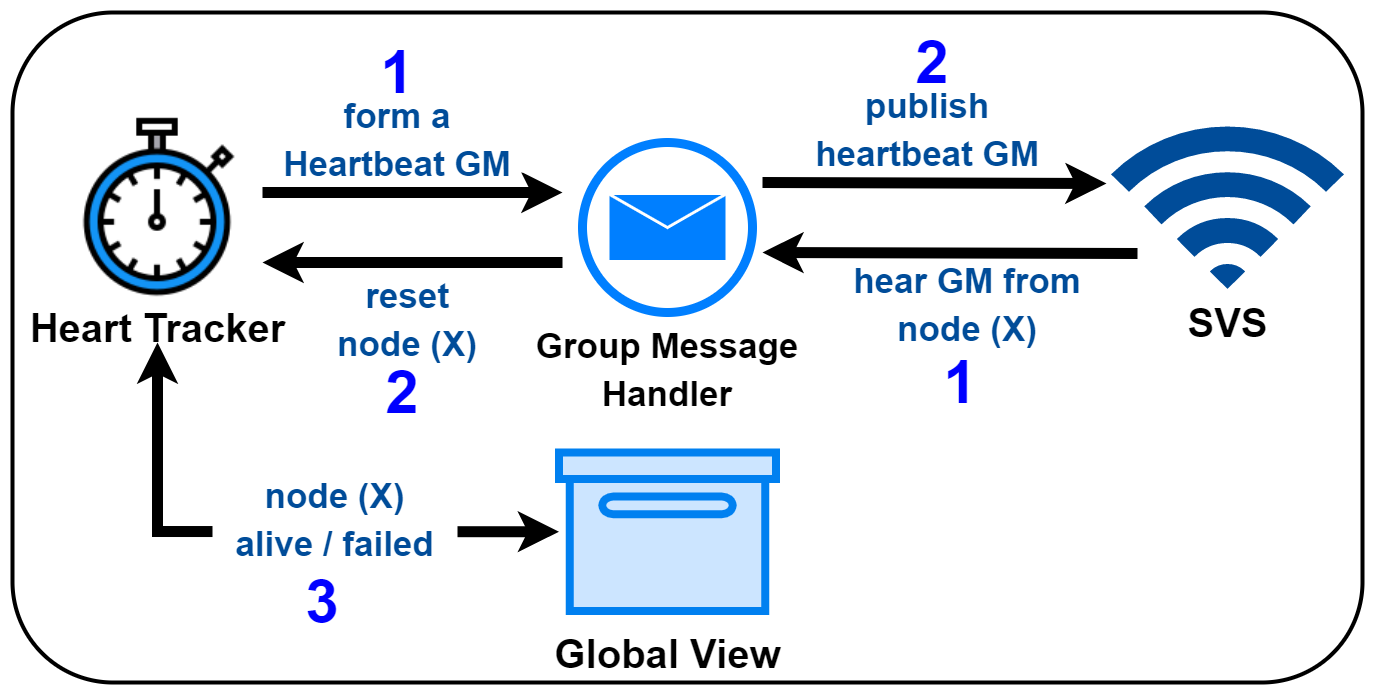
\includegraphics[width=\columnwidth]{visuals/heartbeats-sys.png}
    \caption{Modules Involved with Tracking and Maintaining Node States}
    \label{fig:heartbeats-sys}
\end{figure}

A node becomes unresponsive for the following reasons:

\begin{itemize}
    \item To leave the system a node must remove the hydra infrastructure or shut down. It will become unresponsive and be dropped from the system over time providing the same availability to rejoin that is discussed in 6.5.
    \item An incident occurs that limits communication between two or more nodes, or completely shut down the node.
\end{itemize}

To label a node as unresponsive, a total of three failed heartbeats must be noticed by another nodes heartbeat tracker. The Heartbeats system including the tracker is shown in figure \ref{fig:heartbeats-sys}. All nodes are responsible for their own detection of unresponsive nodes. Once an unresponsive node has been detected, the investigating node will move the unresponsive node to a suspended record of nodes that have gone offline. This status allows the node to update its record for other operations such as managing heartbeats and file replication. No message through State Vector Sync (SVS) or the Global View updating the status of the unresponsive node is sent out over the network by the investigating node.

This is done for two reasons:
\begin{itemize}
    \item First, it allows unresponsive nodes during some disruptions to continue their communication with the rest of the network in the case of a partition. It is also assumed that all other nodes will recognize that a node is unresponsive too if it had truly gone offline. Once the disruption is over the unresponsive node will follow the reestablishment process with the investigating node(s) that have labeled it unresponsive.

    \item Second, if a node has completely gone offline; it can be assumed all other nodes will soon detect this because the offline node will no longer send heartbeats.
\end{itemize}

%\todo[inline]{rephrase}
These two simple assumptions for handling unresponsive nodes cover all situations that could be reached within the system and allow for more accurate detection of disruptions within the system by handling them locally. 
This is done to avoid situations where node A may communicate normally with the rest of the network except for node B. If we did not handle unresponsiveness locally in this case, node B may alert the rest of the network that node A is unresponsive, cutting it off from communicating with the entire network due only to a minor communication problem between node A and B.
%cutting its communication to the entire network due to minor communication issues between it and one other node.

\subsection{Nodes leaving the system}
Nodes at anytime may leave the system as they wish and must simply state it as any other update To leave the system, a node can publish the leave GM or become unresponsive as previously discussed in section \ref{sec:nodes-unresponsive}. The leave GM allows the rest of the system to begin the replication procedure outlined within section \ref{sec:nodes-unresponsive}. This simplifies determining what data needs to be replicated as it can be determined from the leaving node itself, rather the the federation of nodes determining which files. Once the leaving node has determined which files need to be replicated it will publish the leave GM containing this list for the other nodes. Once a leave GM is published the other federation nodes can replicate this list of files received. However, a leaving node is not required to stay for this process, since the federation can recover from it becoming unresponsive. A leaving node deciding to remain throughout the leaving procedure does provide performance benefits to replication as replicas can be obtained from the leaving node.The leaving node will begin replicating files to them based on the favor found within all GMs.

In this formal leaving process it is not necessary for the other nodes to need to determine what files to replicate. They will allow the leaving node to determine this has it already has the knowledge of how many copies of its own files exist, and which need to be replicated. Other federation nodes are on stand by until the leaving node becomes unresponsive or completes the formal leaving process. Once this process is determined complete from store GMs a second leave message will originate from the leaving node to alert the federation of this, and it will complete leaving the system. During this stand by all other federation nodes will move the leaving nodes on list records to the 'on history' records. The leaving node will be listed in the 'on history' for a duration of one month in case the leaving node rejoins the federation. When this month duration expires all records of the left node will be removed from the 'on history'. This allows for temporarily leaving the system but if a node is gone for to long treating it as a new node upon rejoining.

% add the leave group message in group message section
% fully explain full leave message
% detail when this leave message is issued but how other nodes react
% temporary leaves
% keep files on the on list for a duration

\subsection{Reestablishing a Node's State / Node State Reinstatement}
For reinstatement of a node the same name of the node's previous state must be used. This is done to re-link with the records other nodes within the network hold for the previous iteration of our current node. Along with this a local recovery file representing the state in which said node was at the time it became unresponsive or offline is utilized. This file is used locally to determine any differences that have occurred on the system since it last communicated with the Hydra network, and then communicate these differences to the wider network. The purpose of using the differences in system states is that it is more likely by only correcting what is different few corrections will be needed overall, this assumption does dwindle overtime. This process is to allow the node to reclaim its previous status within the network while also updating any nodes that need to know about changes. For example, if a data set was removed during the lapse in communication then other nodes expecting our reinstated node to contain that data need to be alerted to the fact it no longer contains that data. This allows for quick and accurate recovery of a node even if files were deleted or inserted from its system during the lapse in communication.